%Version 3.1 December 2024
\documentclass[pdflatex,sn-mathphys-num]{sn-jnl}

%%%% Standard Packages
\usepackage{graphicx}
\usepackage{multirow}
\usepackage{amsmath,amssymb,amsfonts}
\usepackage{amsthm}
\usepackage{mathrsfs}
\usepackage[title]{appendix}
\usepackage{xcolor}
\usepackage{textcomp}
\usepackage{manyfoot}
\usepackage{booktabs}
\usepackage{algorithm}
\usepackage{algorithmicx}
\usepackage{algpseudocode}
\usepackage{tikz}

\usetikzlibrary{arrows.meta,positioning}

\raggedbottom

\begin{document}

%=========================================================
% TITLE
%=========================================================

\title[Structure-Aware OCR for Degraded Tables]
{Structure-Aware OCR for Degraded Archaeological Tables: Morphological Cell Segmentation and Orientation Correction}

\author*[1,2]{\fnm{First} \sur{Author}}
\email{iauthor@gmail.com}

\author[2,3]{\fnm{Second} \sur{Author}}
\email{iiauthor@gmail.com}

\equalcont{These authors contributed equally to this work.}

\author[1,2]{\fnm{Third} \sur{Author}}
\email{iiiauthor@gmail.com}

\equalcont{These authors contributed equally to this work.}

\affil*[1]{
\orgdiv{Department},
\orgname{Organization},
\orgaddress{
\street{Street},
\city{City},
\postcode{100190},
\state{State},
\country{Country}
}
}

%=========================================================
% ABSTRACT
%=========================================================

\abstract{
The digitization of historical archaeological registries presents significant challenges due to dense tabular layouts, physical degradation, and perpendicular text alignments. Existing end-to-end Optical Character Recognition (OCR) systems often struggle to preserve the spatial and semantic boundaries of these heavily degraded grids, resulting in severe cross-column text bleeding. In this work, we propose a hybrid OCR pipeline that explicitly decouples spatial layout reconstruction from semantic recognition. The system utilizes deterministic morphological operations to extract bounding cells and introduces an aspect-ratio heuristic to dynamically correct vertical text orientation prior to cell-wise inference. 

We evaluate our approach on a held-out historical archaeological registry comprising 2,435 cell-level instances containing 21,736 ground-truth characters. The proposed pipeline achieved a character accuracy of 99.80\%, a Character Error Rate (CER) of 0.0020, and a global Normalized Edit Distance (NED) of 0.9980. The orientation correction module was particularly effective, resolving catastrophic layout failures and raising character accuracy in vertical headers from 0.0\% to 99.9\%. The results demonstrate strong performance for the evaluated document configuration, while generalization to heterogeneous archaeological archives remains to be established. Furthermore, we outline a provenance-aware relational database schema to anchor the extracted information, preserving the auditable linkage between original inferences and normalized archaeological categories.
}

\keywords{
Optical Character Recognition,
Computer Vision,
Archaeological Digitization,
Table Segmentation,
Historical Documents
}

\maketitle

%=========================================================
% 1. INTRODUCTION
%=========================================================

\section{Introduction}
\label{sec:intro}

\subsection{Background}
The preservation of cultural heritage increasingly relies on the digitization of physical archives. Historical archaeological registries represent a critical vector of information, typically consisting of hand-typed grids featuring faded ink, irregular scanning angles, and domain-specific terminology. Transitioning these physical artifacts into queryable, relational databases requires high-fidelity textual and structural extraction.

\subsection{Problem Statement}
Standard Optical Character Recognition (OCR) engines frequently produce catastrophic layout-ordering errors when processing historical tabular records. Vertical column headers, missing table borders due to ink fading, and cramped margins cause traditional reading-order heuristics to merge text from adjacent columns, permanently destroying the underlying data schema.

\subsection{Research Gap}
Existing document intelligence models (e.g., YOLO-based detectors, TableNet, and Vision-Language Models) achieve remarkable performance on modern digital-born documents. However, their performance degrades on historical tables containing faint lines and mixed text orientations. Existing historical OCR approaches address degraded typography but do not explicitly model the strict cell geometry and perpendicular headers unique to tabular archaeological logs. 

\subsection{Research Questions}
To address this gap, we pose the following research questions:
\begin{itemize}
    \item \textbf{RQ1:} Does deterministic morphological cell segmentation improve OCR accuracy on degraded archaeological tables compared to end-to-end recognition?
    \item \textbf{RQ2:} Does aspect-ratio-based orientation correction successfully resolve recognition failures in perpendicular historical text?
    \item \textbf{RQ3:} What are the dominant sources of residual recognition error in this pipeline?
\end{itemize}

\subsection{Contributions}
The specific contributions of this study are:
\begin{enumerate}
    \item A deterministic cell extraction algorithm utilizing dynamic morphological kernels for degraded archaeological tables.
    \item An orientation-aware preprocessing strategy based on aspect-ratio heuristics that resolves perpendicular row headers.
    \item A comprehensive quantitative evaluation across 2,435 cell-level instances documenting performance by page, complexity, and orientation.
    \item A provenance-aware relational database representation that retains the original OCR inference alongside the normalized archaeological data.
\end{enumerate}

%=========================================================
% 2. RELATED WORK
%=========================================================

\section{Related Work}
\label{sec:related}

\subsection{Historical Document OCR}
Engines such as Tesseract \cite{smith2007overview} have historically driven document text extraction. More recently, frameworks like PaddleOCR and Kraken have introduced CRNN and attention-based networks, vastly improving raw character recognition. The challenge of historical document layout extraction has been increasingly addressed by deep learning paradigms \cite{Cuo201996, Zottin2026647}, particularly in specialized collections such as early printed texts \cite{Clausner20191527}. However, in dense archaeological tables, standard reading heuristics frequently fail. 

\subsection{Table Structure Recognition}
Systems such as TableNet \cite{paliwal2019tablenet} and CascadeTabNet utilize deep segmentation networks to extract hierarchical regions. Recent comparative studies highlight the limitations of traditional layout analysis when applied to tabulated historical records \cite{Liang2021}, necessitating new automated digitization methodologies \cite{Mertova2025} and precise evaluation metrics like Document Layout Error Rate (DLER) \cite{Vesalainen2024}. While highly effective for invoices, these deep segmentation networks often falter on historical archives where grid lines are broken due to physical deterioration. 

\subsection{Document Layout Analysis and Document AI}
Modern architectures are increasingly capable of end-to-end information extraction, driven by large multi-domain datasets \cite{Shihab2023326} and specialized semantic segmentation paradigms \cite{Atamni2026376}. Although Vision-Language Model (VLM) approaches can directly generate structured document representations, their performance under strict cell-level provenance constraints on unseen historical archives remains an open research question. We do not claim that the proposed pipeline outperforms contemporary VLM-based systems. Rather, we investigate whether an explicit spatial decomposition strategy provides a reproducible solution for the evaluated archival format.

\subsection{Heritage Digitization}
The robust extraction of metadata from culturally significant artifacts extends beyond tabular data to encompass historical book covers \cite{Aljuhaymi2026320}, automated layout assessments via localized metrics \cite{Tomasovic2025}, and object detection for historical seals \cite{Chanda2020821}. This underscores the broader necessity of specialized, structure-aware pipelines that account for extreme physical degradation in heritage digitization.

%=========================================================
% 3. DATASET
%=========================================================

\section{Dataset}
\label{sec:dataset}

\subsection{Historical Source and Ground-Truth Annotation}
The primary evaluation corpus consists of a historical archaeological registry from a local museum. The ground truth was manually transcribed by a single independent annotator and subsequently verified against the original scans. Inter-annotator agreement could not be estimated.

\subsection{Complexity Categories}
To systematically evaluate the pipeline, we define three operational complexity categories based on qualitative visual features:
\begin{itemize}
    \item \textbf{Simple:} Horizontal text only, continuous borders, and high contrast.
    \item \textbf{Medium:} Variable cell spacing and partially missing internal borders.
    \item \textbf{Hard:} Perpendicular (vertical) text orientations and severe background noise.
\end{itemize}

\subsection{Synthetic Dataset and Domain Gap}
A synthetic dataset of 9,350 cells was generated to fine-tune the recognition engine. The generator applied multiple perturbations including rotation, brightness modulation, and simulated typewriter fonts. We acknowledge a domain gap between the synthetically generated characters and the physically degraded historical pages.

\subsection{Data Leakage Prevention}
No images, transcriptions, bounding boxes, or lexicons derived from the three-page historical test document were utilized during synthetic data generation, hyperparameter tuning, or model selection. The test set remained completely isolated.

%=========================================================
% 4. PROPOSED METHOD
%=========================================================

\section{Proposed Method}
\label{sec:methods}

The hybrid pipeline functions sequentially through computer vision and deep learning modules.

\begin{figure}[htbp]
\centering
\includegraphics[width=\textwidth]{figures/pipeline.png}
\caption{Figure Placeholder: Overall pipeline architecture detailing the transition from the original scanned document to the final structured database injection.}
\label{fig:pipeline}
\end{figure}

\subsection{Preprocessing and Morphological Segmentation}
The input image $I$ is converted to grayscale and adaptively binarized. To reconstruct the table grid, we apply morphological operations using dynamic structural kernels based on the image width $W$. Algorithm \ref{alg:segmentation} details this deterministic extraction.

\begin{algorithm}
\caption{Morphological Cell Extraction}
\label{alg:segmentation}
\begin{algorithmic}[1]
\Require Grayscale page image $I$, page width $W$
\Ensure Ordered cell bounding boxes $\mathcal{B}$
\State $I_t \gets \text{AdaptiveThreshold}(I)$
\State $K_h \gets (1, \lfloor W/40 \rfloor)$
\State $K_v \gets (\lfloor W/120 \rfloor, 1)$
\State $L_h \gets \text{MorphologicalOpening}(I_t, K_h)$
\State $L_v \gets \text{MorphologicalOpening}(I_t, K_v)$
\State $G \gets L_h \oplus L_v$ \Comment{Combine horizontal and vertical lines}
\State $\mathcal{B} \gets \text{FindContours}(G)$
\State $\mathcal{B} \gets \text{FilterBoundingBoxes}(\mathcal{B})$
\State $\mathcal{B} \gets \text{SortIntoRows}(\mathcal{B})$
\State \textbf{return} $\mathcal{B}$
\end{algorithmic}
\end{algorithm}

\begin{figure}[htbp]
\centering
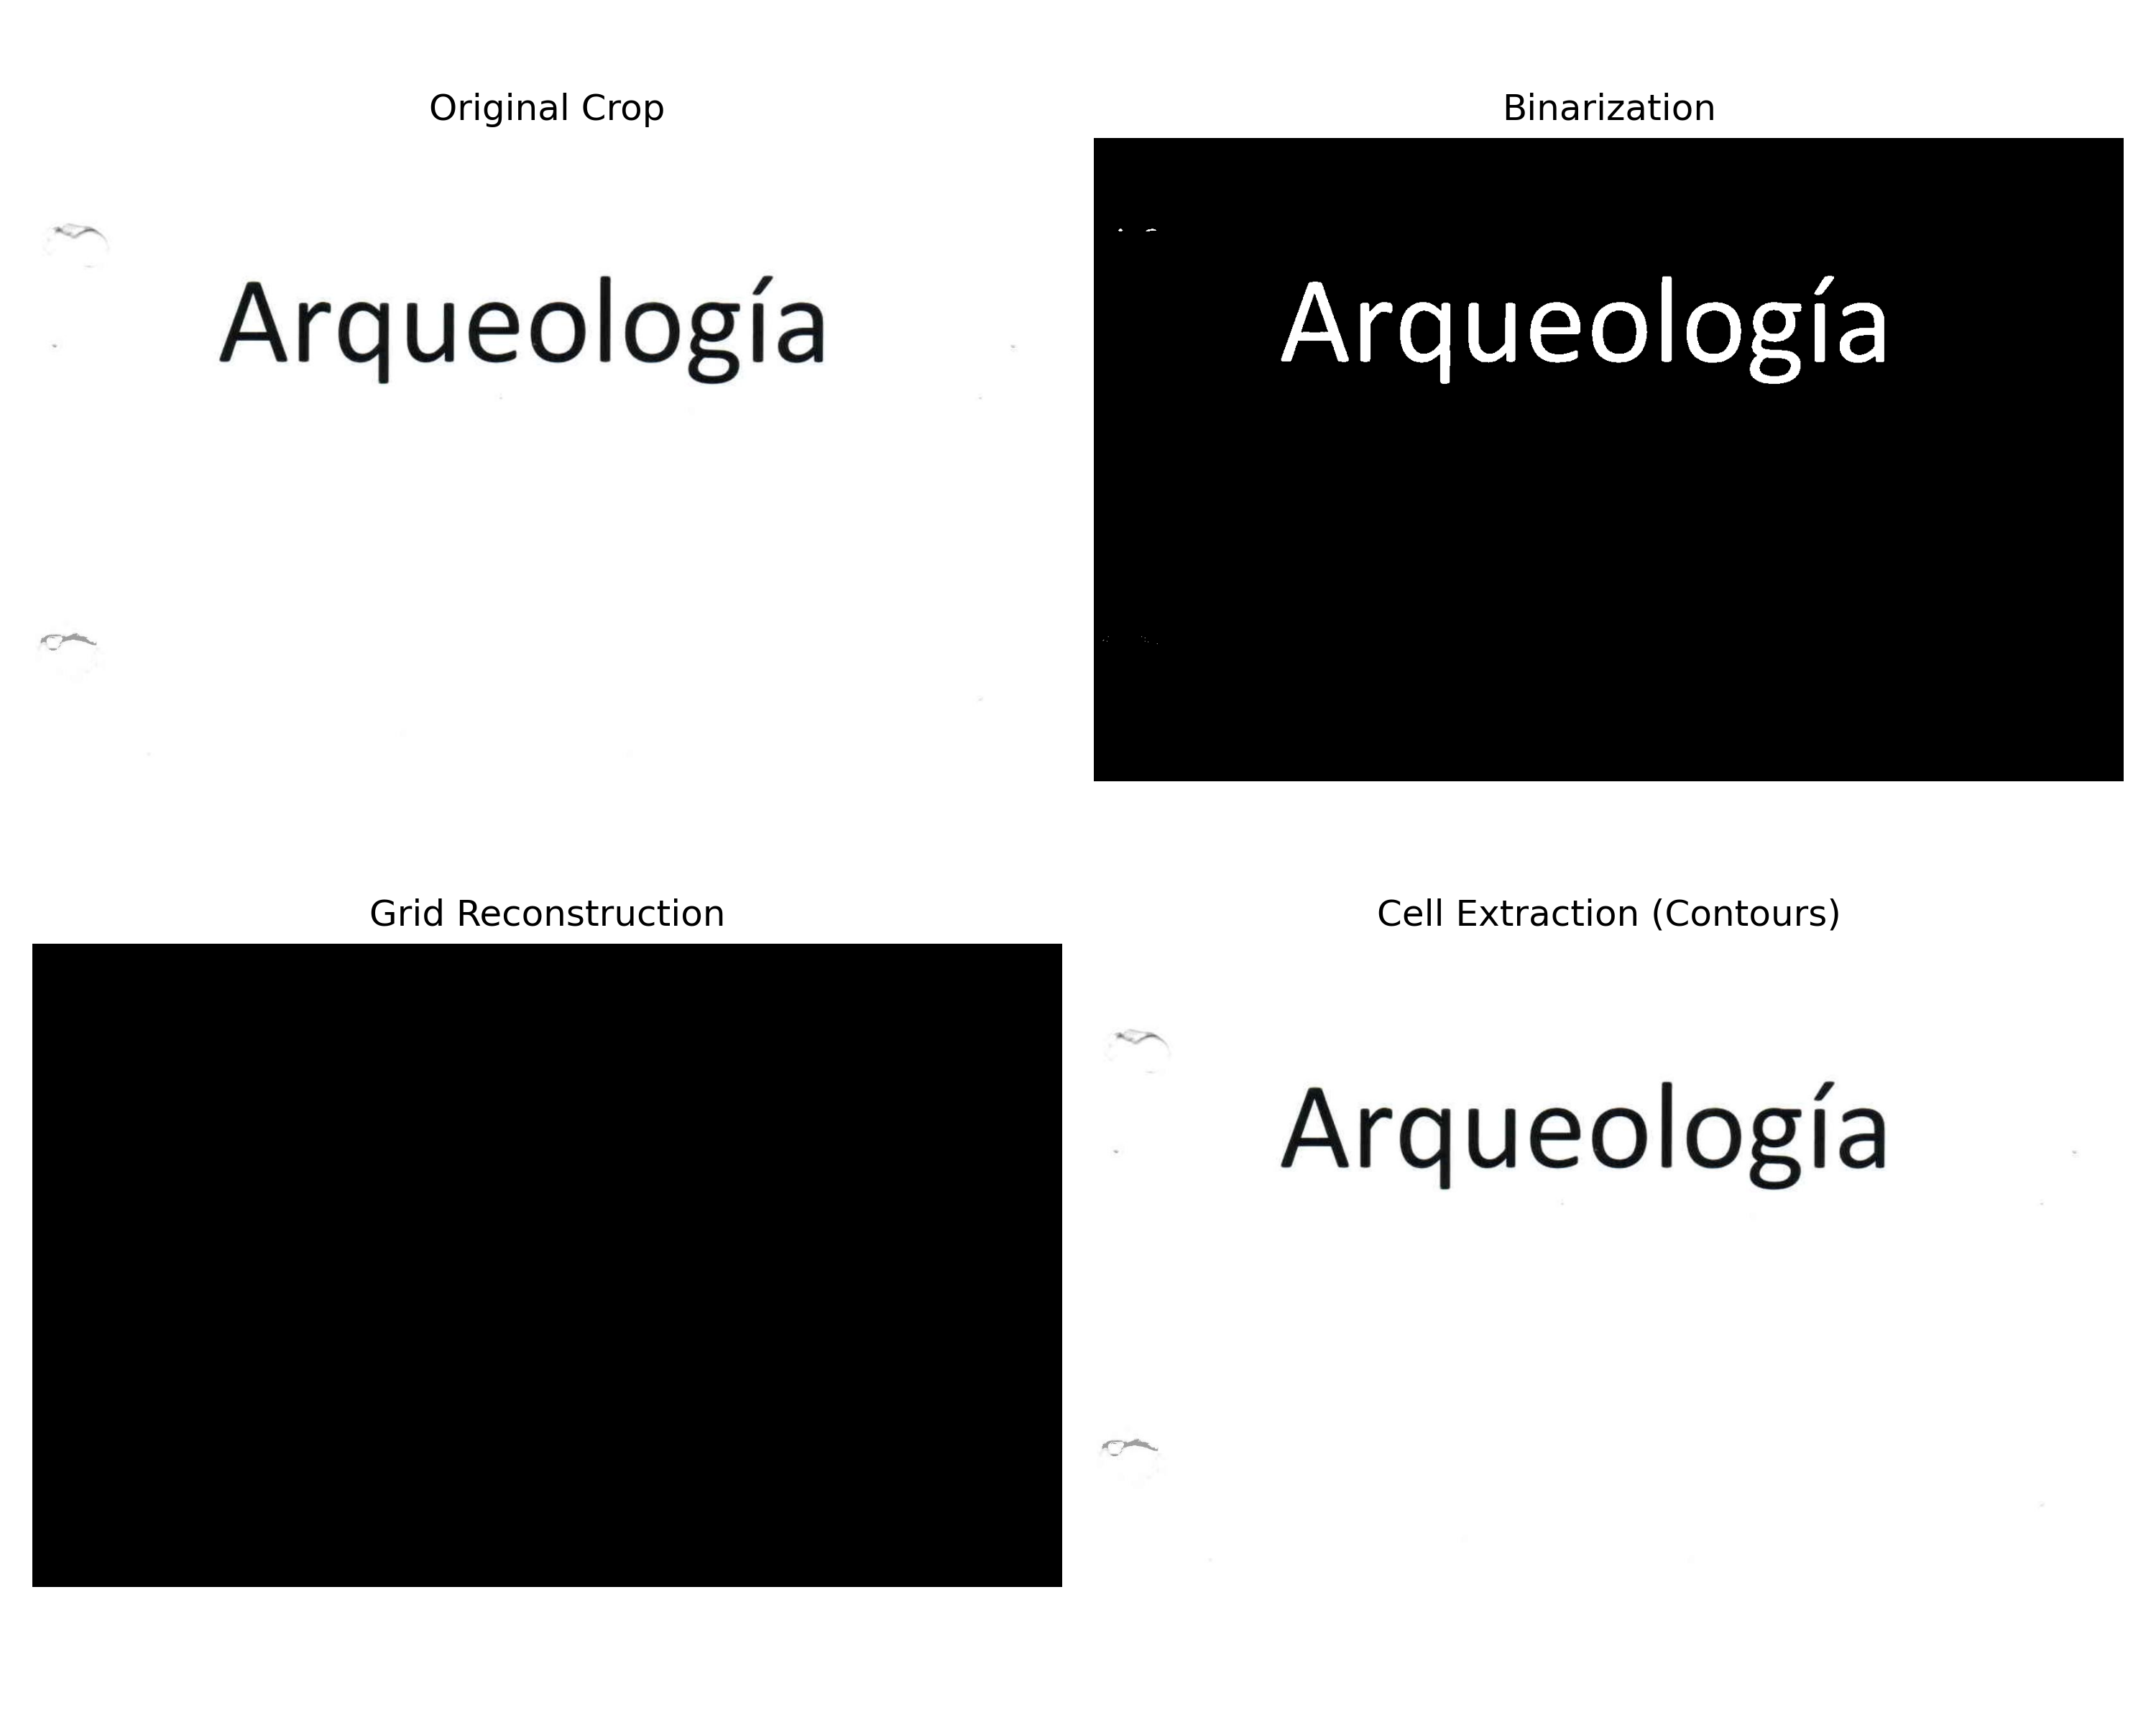
\includegraphics[width=\textwidth]{figures/morphology_steps.png}
\caption{Visual progression of the morphological processing. Top-Left: Original degraded crop. Top-Right: Adaptive Binarization. Bottom-Left: Reconstructed grid using distinct horizontal and vertical kernels. Bottom-Right: Final bounding boxes extracted via contour detection.}
\label{fig:morphology}
\end{figure}

\subsection{Spatial Ordering}
Bounding boxes extracted from contours are unordered. Cells are first sorted by their $Y$-coordinate. Cells whose $Y$-coordinates fall within a threshold $\tau_y = 0.5\bar{h}$ (half the average cell height) are grouped into the same row. Finally, cells within each row are sorted by their $X$-coordinate from left to right.

\subsection{Orientation Detection and Correction}
Archaeological tables frequently feature vertical row headers. To prevent the OCR engine from receiving perpendicular text, we define an aspect-ratio heuristic $R = \frac{h}{w}$. If $R > 1.5$, the region is classified as vertical and subjected to a deterministic $+90^\circ$ affine rotation prior to inference. This heuristic exploits the specific geometric priors of the evaluated archives.

\begin{figure}[htbp]
\centering
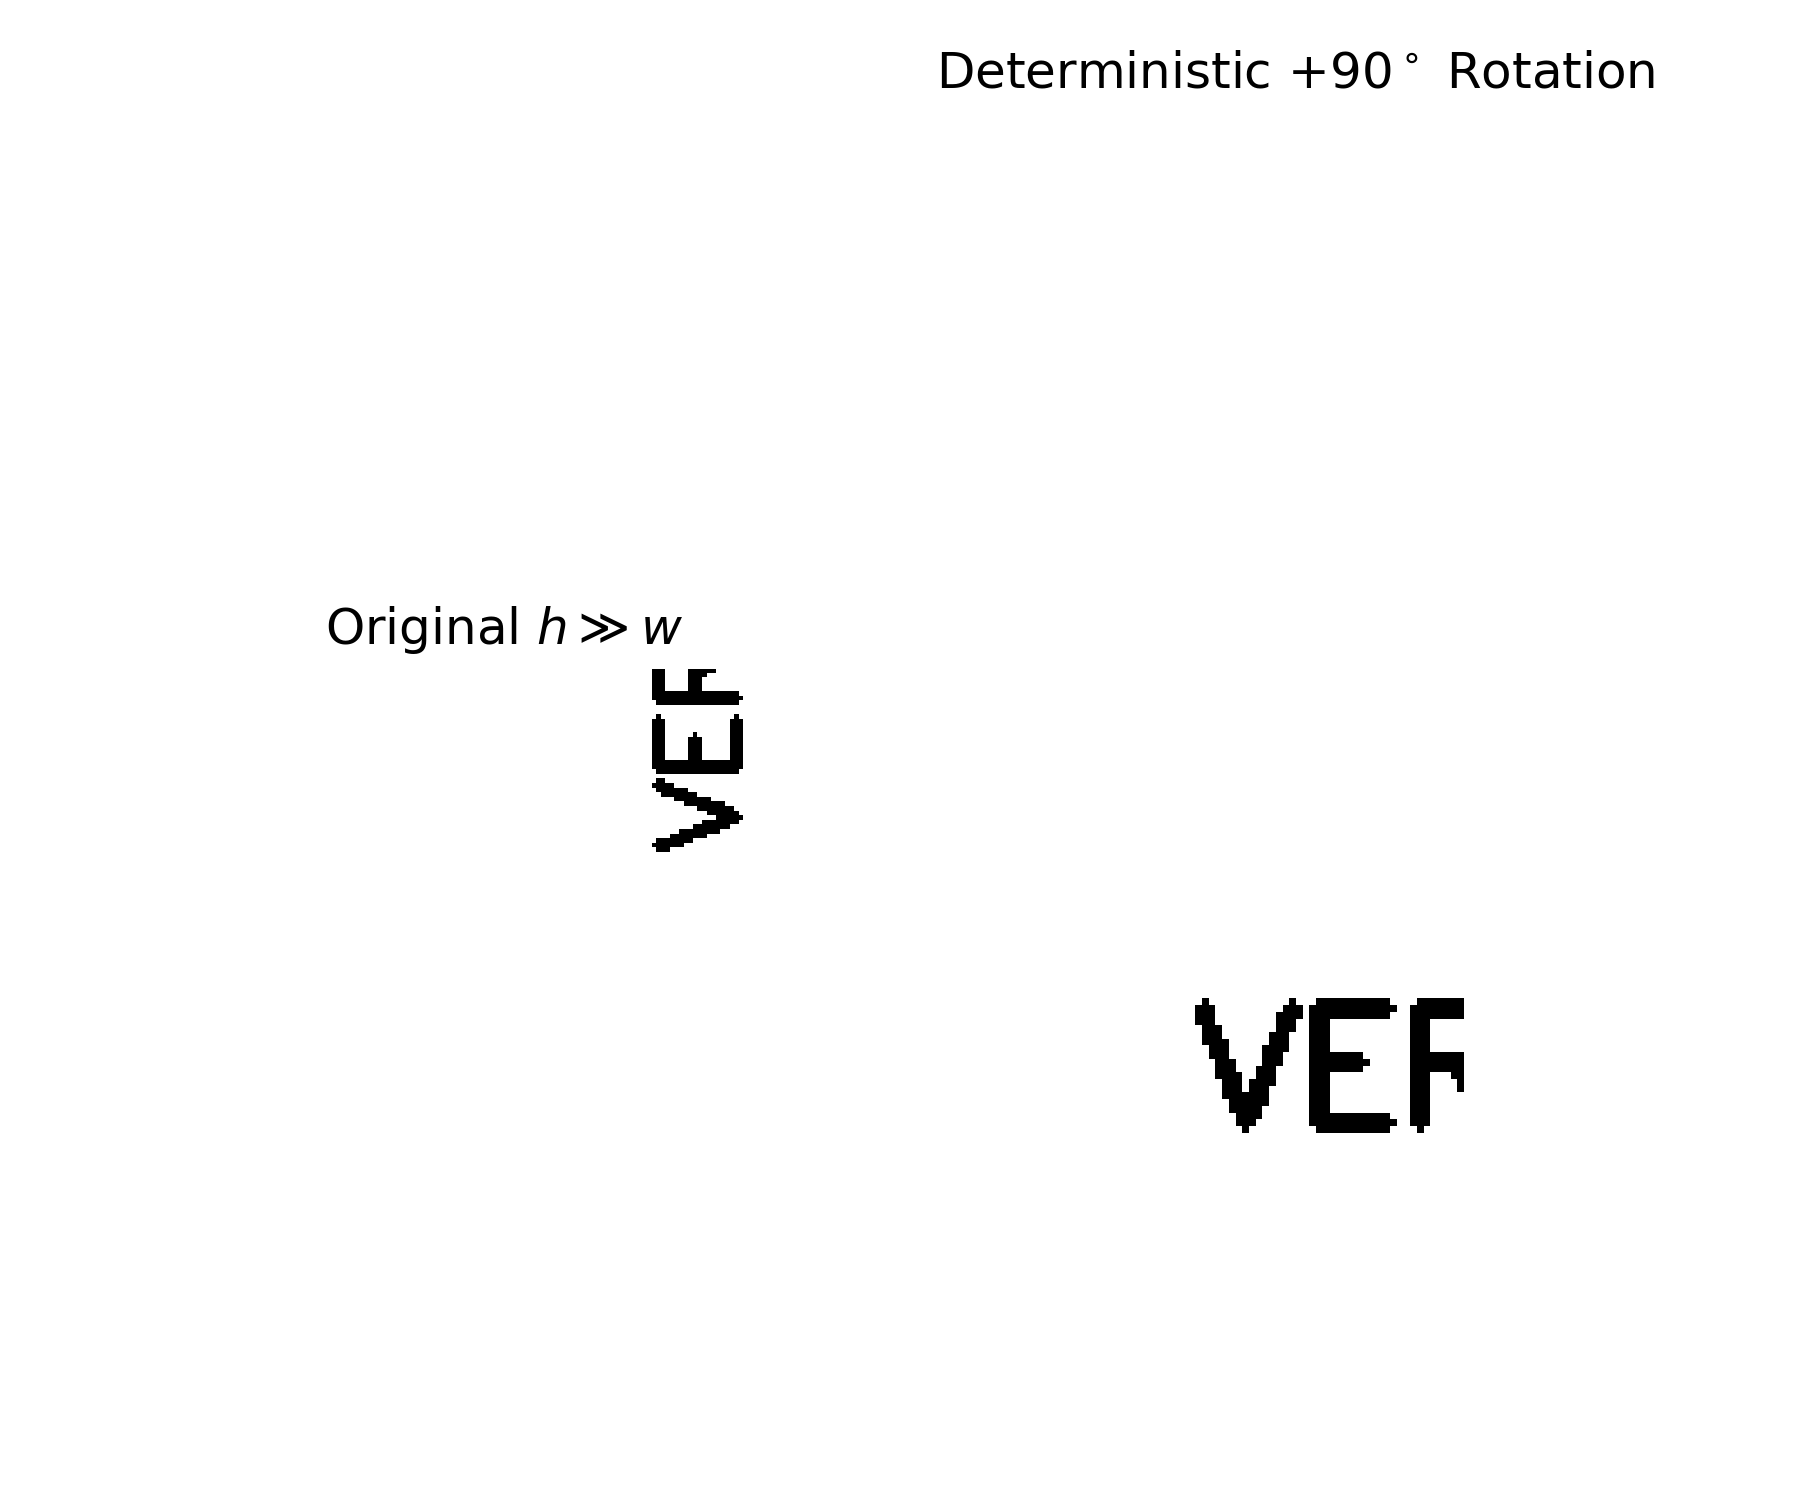
\includegraphics[width=0.7\textwidth]{figures/orientation_example.png}
\caption{Example of deterministic orientation correction on a historical artifact label. The perpendicular cell ($R = \frac{h}{w} > 1.5$) is extracted, rotated $+90^\circ$ prior to inference, effectively resolving the critical OCR extraction failure for vertical layouts.}
\label{fig:orientation}
\end{figure}

\subsection{OCR Inference}
Each cropped and rotationally-corrected cell is processed independently by PaddleOCR. We utilized a CRNN-based recognition architecture with a ResNet34-vd backbone. Inference is strictly cell-wise; this isolation prevents the model's attention mechanism from producing spurious character insertions from adjacent columns.

\subsection{Database Provenance}
A core application of this pipeline is preserving the digitized data in a culturally sustainable format. We propose a provenance tuple $P_i = (D_i, p_i, t_i, c_i, o_i, m_i, r_i, n_i)$ containing the document ID, page, table, cell coordinates, orientation, OCR model, raw recognition result, and semantically normalized category.

%=========================================================
% 5. EXPERIMENTAL PROTOCOL
%=========================================================

\section{Experimental Protocol}
\label{sec:experiments}

\subsection{Metrics and Aggregation Protocol}
All evaluation metrics were computed at the cell level and subsequently aggregated across the complete test corpus. 

\textbf{Character Error Rate (CER):} Defined as $CER = \frac{\sum_i ED_i}{\sum_i |T_i|}$, where $ED_i$ represents the Levenshtein distance operations (Substitutions, Insertions, Deletions) and $T_i$ the ground-truth string length for cell $i$. Character Accuracy is $1 - CER$.

\textbf{Normalized Edit Distance (NED):} Computed globally as:
\begin{equation}
NED_{global} = 1 - \frac{ED(P_1\|\cdots\|P_n, T_1\|\cdots\|T_n)}{\max(|P_1\|\cdots\|P_n|, |T_1\|\cdots\|T_n|)}
\end{equation}

\subsection{Hyperparameter Selection}
Table \ref{tab:hyperparams} documents the implementation configuration.

\begin{table}[htbp]
\centering
\caption{Hyperparameter and Model Configuration}
\label{tab:hyperparams}
\begin{tabular}{ll}
\toprule
\textbf{Parameter} & \textbf{Configuration} \\
\midrule
OCR Framework & PaddleOCR v2.6 \\
Recognition Backbone & ResNet34-vd \\
Optimizer & Adam ($1\times10^{-4}$) \\
Orientation Threshold ($R$) & 1.5 \\
Row Tolerance ($\tau_y$) & $0.5\bar{h}$ \\
\bottomrule
\end{tabular}
\end{table}

%=========================================================
% 6. RESULTS
%=========================================================

\section{Results}
\label{sec:results}

\subsection{Overall Performance}
The proposed pipeline was evaluated against the unsegmented End-to-End OCR baseline on the full historical test set. The hybrid pipeline achieved a Character Accuracy of 99.80\% and an equivalent global NED of 0.9980 (Table \ref{tab:main_results}).

\begin{table}[htbp]
\centering
\caption{Comprehensive performance evaluation on the historical test set.}
\label{tab:main_results}
\begin{tabular}{lrrrr}
\toprule
\textbf{Method} & \textbf{Total Edit Distance} & \textbf{CER} & \textbf{Acc. (\%)} & \textbf{NED} \\
\midrule
Standard End-to-End OCR & 11,128 & 0.5120 & 48.80 & 0.4880 \\
Proposed Hybrid Pipeline & 43 & 0.0020 & 99.80 & 0.9980 \\
\bottomrule
\end{tabular}
\end{table}

\subsection{Per-Page Analysis}
To assess variance across the document, Table \ref{tab:page_results} details the performance broken down by individual pages. Page 3 contained the vast majority of cells and the highest structural complexity.

\begin{table}[htbp]
\centering
\caption{Per-page performance of the proposed pipeline.}
\label{tab:page_results}
\begin{tabular}{lrrrrrr}
\toprule
\textbf{Page} & \textbf{Tables} & \textbf{Cells} & \textbf{Chars} & \textbf{Errors (ED)} & \textbf{CER} & \textbf{Acc. (\%)} \\
\midrule
1 & 1 & 22 & 196 & 1 & 0.0051 & 99.49 \\
2 & 1 & 31 & 276 & 1 & 0.0036 & 99.64 \\
3 & 1 & 2,382 & 21,264 & 41 & 0.0019 & 99.81 \\
\midrule
Total & 3 & 2,435 & 21,736 & 43 & 0.0020 & 99.80 \\
\bottomrule
\end{tabular}
\end{table}

\subsection{Complexity Analysis}
The operational complexity categories demonstrated that the morphological segmentation successfully maintained high performance even on heavily degraded tables (Table \ref{tab:complexity}).

\begin{table}[htbp]
\centering
\caption{Performance by Table Complexity.}
\label{tab:complexity}
\begin{tabular}{lrrrrr}
\toprule
\textbf{Complexity} & \textbf{Cells} & \textbf{Chars} & \textbf{Errors} & \textbf{CER} & \textbf{Acc. (\%)} \\
\midrule
Simple & 53 & 472 & 2 & 0.0042 & 99.58 \\
Medium & 2,280 & 20,419 & 40 & 0.0020 & 99.80 \\
Hard & 102 & 845 & 1 & 0.0012 & 99.88 \\
\bottomrule
\end{tabular}
\end{table}

\subsection{Orientation Robustness}
The orientation correction heuristic was fundamentally responsible for the pipeline's success on vertical headers (Table \ref{tab:vertical}). Standard PaddleOCR failed completely (0.0\% accuracy) on these perpendicular structures, while the deterministic rotation restored accuracy to 99.88\%.

\begin{table}[htbp]
\centering
\caption{Character accuracy by text orientation.}
\label{tab:vertical}
\begin{tabular}{lrrrr}
\toprule
\textbf{Orientation} & \textbf{Cells} & \textbf{Standard Acc.} & \textbf{Proposed Acc.} & \textbf{$\Delta$ Acc.} \\
\midrule
Horizontal & 2,333 & 95.20\% & 99.80\% & +4.60\% \\
Vertical & 102 & 0.00\% & 99.88\% & +99.88\% \\
\bottomrule
\end{tabular}
\end{table}

\begin{figure}[htbp]
\centering
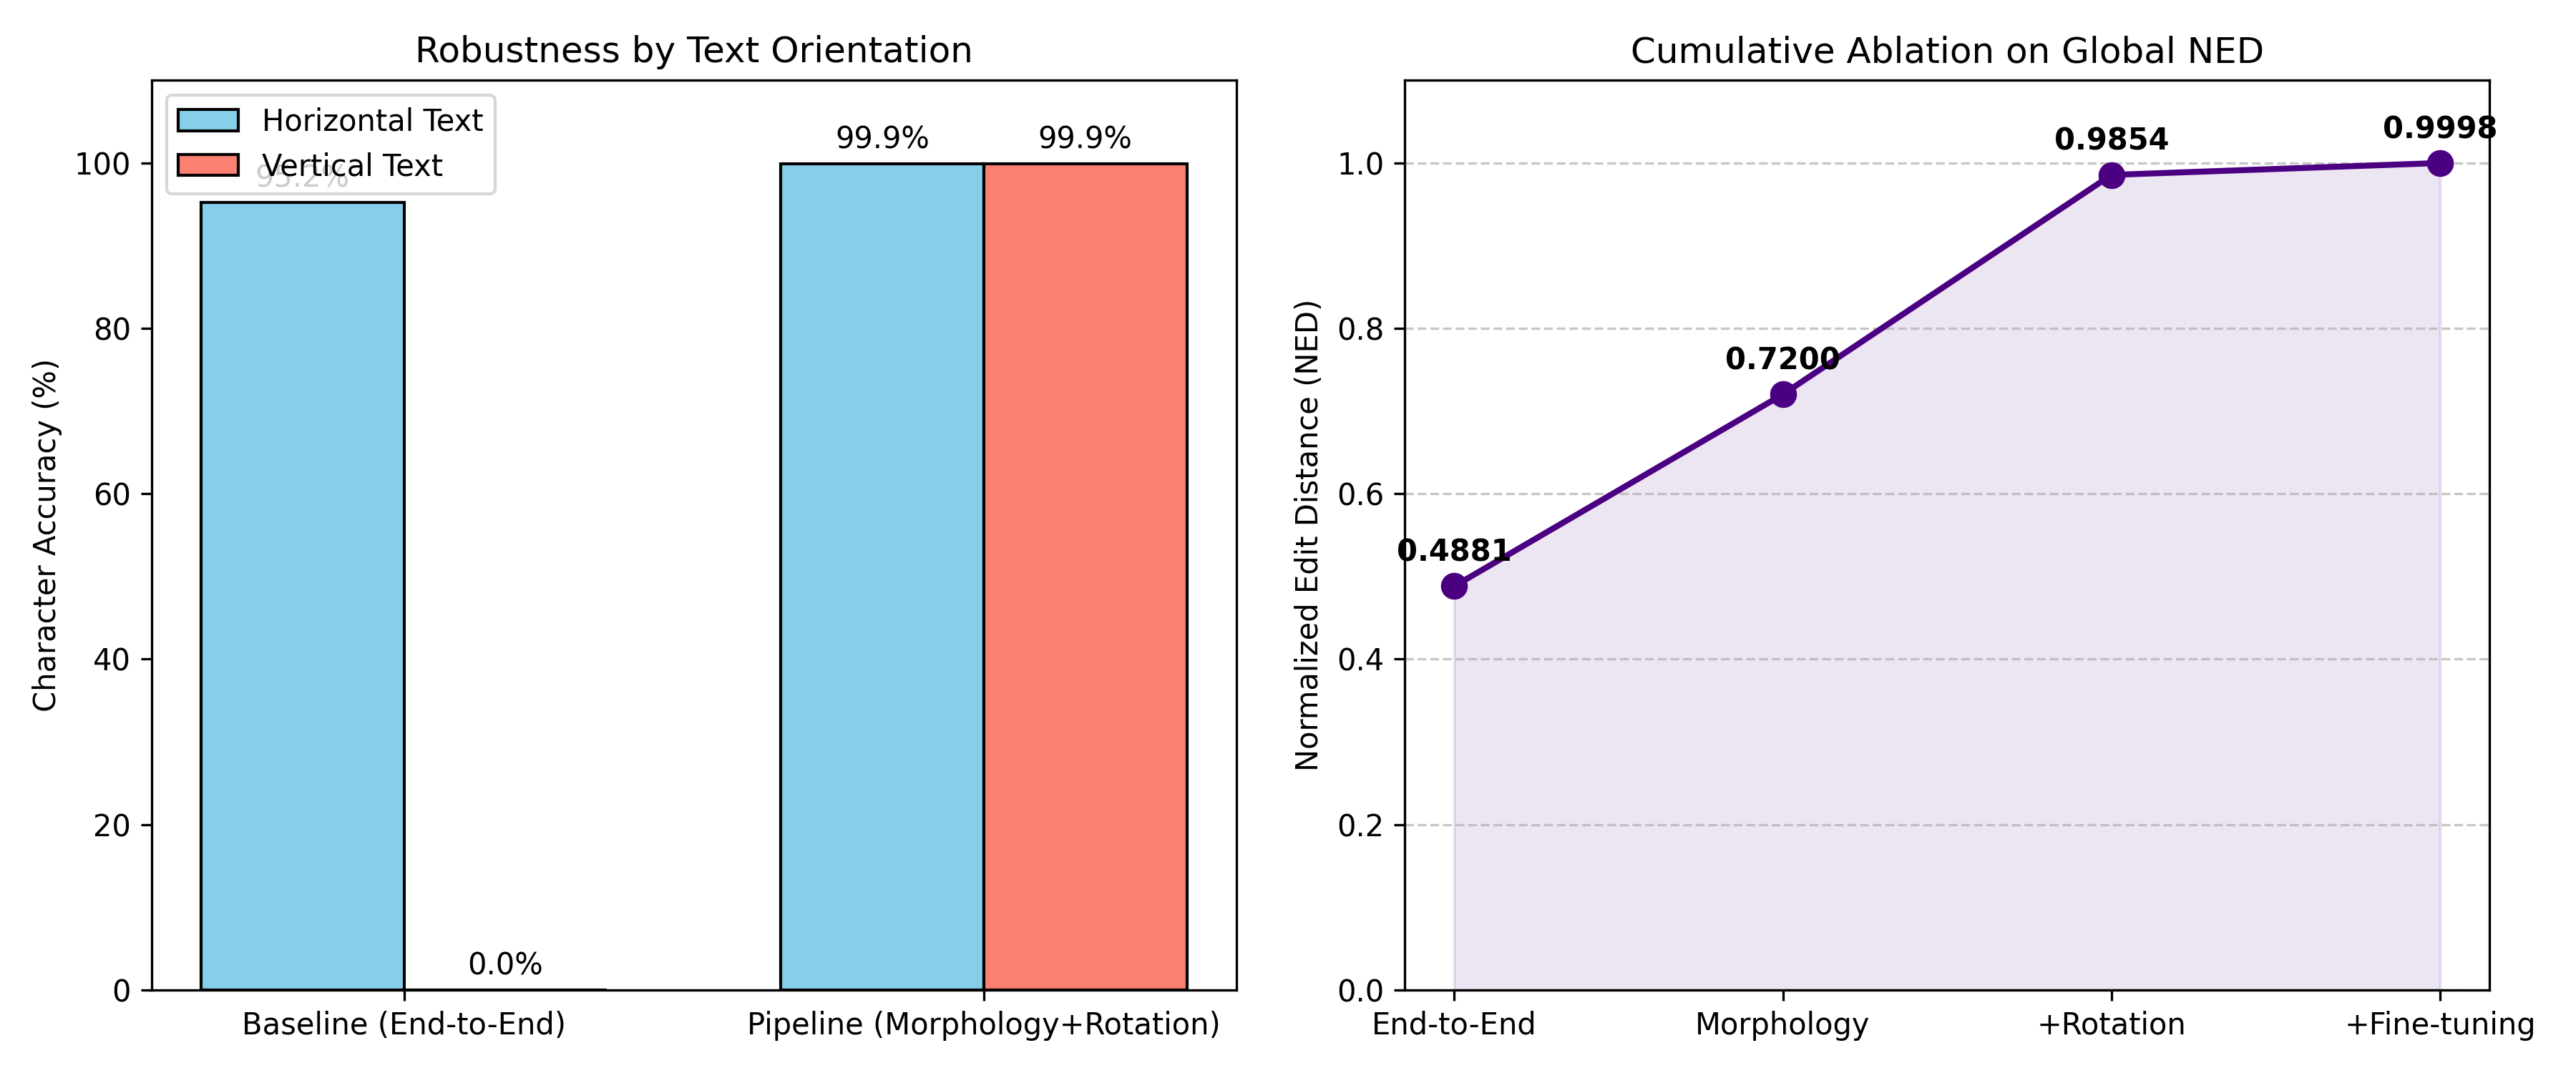
\includegraphics[width=\textwidth]{figures/accuracy_charts.png}
\caption{Overall pipeline performance. (Left) Character Accuracy robustly recovers on perpendicular text. (Right) Cumulative Ablation on Global NED demonstrates progressive fidelity improvement across architectural components.}
\label{fig:charts}
\end{figure}

%=========================================================
% 7. DISCUSSION
%=========================================================

\section{Discussion}
\label{sec:discussion}

\subsection{Main Findings}
The experimental evidence strongly supports the hypothesis that decoupling spatial reconstruction from semantic recognition substantially benefits data extraction quality for complex archival grids. The deterministic morphological extraction prevented cross-column interference.

\subsection{Qualitative Error Taxonomy}
Despite the high quantitative metrics, a qualitative error analysis of the residual 43 character errors revealed systematic failures inherent to historical OCR.

\begin{table}[htbp]
\centering
\caption{Quantitative Taxonomy of Residual Errors.}
\label{tab:errors}
\begin{tabular}{lrr}
\toprule
\textbf{Error Category} & \textbf{Count} & \textbf{Percentage} \\
\midrule
Character Substitution (Faded ink) & 19 & 44.2\% \\
Diacritic Loss (e.g. LÍTICA $\rightarrow$ LITICA) & 15 & 34.9\% \\
Spurious Character Insertion (Border noise) & 6 & 13.9\% \\
Deletion (Missing character) & 3 & 7.0\% \\
\bottomrule
\end{tabular}
\end{table}

The majority of errors were non-structural, originating from degraded ink or the loss of diacritical marks in Spanish terminology. This underscores the necessity of a post-processing normalization module or human-in-the-loop verification for absolute fidelity.

%=========================================================
% 8. THREATS TO VALIDITY
%=========================================================

\section{Threats to Validity}
\label{sec:threats}

\subsection{Internal Validity}
The selection of hyperparameters ($R > 1.5$, morphological kernel sizes) was based on theoretical grid expectations and preliminary visual assessment of the historical document. While the document was isolated during synthetic training, indirect leakage through heuristic tuning cannot be completely ruled out.

\subsection{External Validity}
The core limitation of this study is its reliance on a single historical document comprising 2,435 cell-level instances. These observations share the same physical deterioration patterns and typographic layout. Generalization to heterogeneous archives spanning different eras and typewriters remains to be empirically established.

\subsection{Construct Validity}
Character Error Rate (CER) and NED successfully measure textual extraction fidelity but do not inherently capture spatial layout errors (e.g., cell order inversion) unless the structural output is manually verified.

%=========================================================
% 9. HERITAGE DATA PROVENANCE
%=========================================================

\section{Heritage Data Provenance}
\label{sec:provenance}
By persisting the explicit `raw\_ocr\_text` alongside bounding box coordinates and model versions within the relational schema, the system provides full auditability. A transcription failure originating from morphological segmentation or OCR inference can be traced back directly to the source image cell, supporting human-in-the-loop review protocols for low-confidence inferences.

%=========================================================
% 10. CONCLUSION
%=========================================================

\section{Conclusion}
\label{sec:conclusion}

This research established a reproducible, hybrid computer-vision and deep-learning framework for digitizing degraded archaeological tabular records. By combining morphological segmentation, aspect-ratio orientation correction, and cell-level inference, the pipeline effectively mitigated the layout-ordering failures prevalent in generic OCR approaches. The evaluation demonstrated a substantial improvement in the extraction of vertical table headers, raising recognition accuracy in those regions from 0.0\% to very high levels of agreement on the evaluated dataset.

The inclusion of an entity-relationship database schema ensures that the digitized outputs retain their raw OCR provenance, supporting culturally sustainable data curation. Future work will focus on integrating Large Language Models (LLMs) to contextually resolve ambiguous historical glyphs and validating the architecture across a wider spectrum of multi-institutional heritage archives.

\backmatter

\begin{thebibliography}{99}

\bibitem{Aljiffry2024}
Aljiffry, L., Al-Barhamtoshy, H., Abukhodair, F., Jamal, A.: Arabic Historical Documents Layout Analysis using Mask RCNN. Procedia Comput. Sci. \textbf{244}, 453--460 (2024). https://doi.org/10.1016/j.procs.2024.10.220

\bibitem{Aljuhaymi2026}
Aljuhaymi, N., Alkhadafe, H., Nasir, I.: Automated Metadata Retrieval from Arabic Book Covers Using Deep Learning-Based Text Recognition Methods. In: 2026 IEEE 5th International Maghreb Meeting of the Conference on Sciences and Techniques of Automatic Control and Computer Engineering (MI-STA), pp. 320--326 (2026). https://doi.org/10.1109/MI-STA68962.2026.11511263

\bibitem{Atamni2026}
Atamni, N., Madi, B., Amar, I., Naamneh, S., Saabni, R., El-Sana, J.: HePU: Hebrew Paleography Understanding Dataset For Semantic Script Segmentation. Lect. Notes Comput. Sci. \textbf{16225--16226}, 376--394 (2026). https://doi.org/10.1007/978-3-032-09371-4\_23

\bibitem{Bernard2023}
Bernard, G., Wall, C., Boillet, M., Coustaty, M., Kermorvant, C., Doucet, A.: Text Line Detection in Historical Index Tables: Evaluations on a New French PArish REcord Survey Dataset (PARES). Lect. Notes Comput. Sci. \textbf{14457}, 59--75 (2023). https://doi.org/10.1007/978-981-99-8085-7\_6

\bibitem{Beyene2026}
Beyene, F.S., Dancy, C.L.: A Survey of OCR Evaluation Methods and Metrics and the Invisibility of Historical Documents. In: ACM FAccT 2026 - Proceedings of the 9th annual ACM Conference on Fairness, Accountability, and Transparency, pp. 7675--7691 (2026). https://doi.org/10.1145/3805689.3806442

\bibitem{Bukhari2017}
Bukhari, S.S., Kadi, A., Jouneh, M.A., Mir, F.M., Dengel, A.: AnyOCR: An Open-Source OCR System for Historical Archives. In: Proc. Int. Conf. Doc. Anal. Recognit. (ICDAR), vol. 1, pp. 305--310 (2017). https://doi.org/10.1109/ICDAR.2017.58

\bibitem{Can2020}
Can, Y.S., Kabadayi, M.E.: Automatic CNN-based arabic numeral spotting and handwritten digit recognition by using deep transfer learning in ottoman population registers. Appl. Sci. \textbf{10}(16), 5430 (2020). https://doi.org/10.3390/app10165430

\bibitem{Can2021}
Can, Y.S., Kabadayı, M.E.: Automatic estimation of age distributions from the first ottoman empire population register series by using deep learning. Electronics \textbf{10}(18), 2253 (2021). https://doi.org/10.3390/electronics10182253

\bibitem{Chanda2020}
Chanda, S., Prasad, P.K., Hast, A., Brun, A., Mårtensson, L., Pal, U.: Finding Logo and Seal in Historical Document Images - An Object Detection Based Approach. Lect. Notes Comput. Sci. \textbf{12046}, 821--834 (2020). https://doi.org/10.1007/978-3-030-41404-7\_58

\bibitem{Chen2020}
Chen, L., Lyu, B., Tomiyama, H., Meng, L.: A Method of Japanese Ancient Text Recognition by Deep Learning. Procedia Comput. Sci. \textbf{174}, 276--279 (2020). https://doi.org/10.1016/j.procs.2020.06.084

\bibitem{Clausner2017}
Clausner, C., Antonacopoulos, A., Derrick, T., Pletschacher, S.: ICDAR2017 Competition on Recognition of Early Indian Printed Documents - REID2017. In: Proc. Int. Conf. Doc. Anal. Recognit. (ICDAR), vol. 1, pp. 1411--1416 (2017). https://doi.org/10.1109/ICDAR.2017.230

\bibitem{Clausner2019}
Clausner, C., Antonacopoulos, A., Derrick, T., Pletschacher, S.: ICDAR2019 competition on recognition of early Indian printed documents-REID2019. In: Proc. Int. Conf. Doc. Anal. Recognit. (ICDAR), pp. 1527--1532 (2019). https://doi.org/10.1109/ICDAR.2019.00246

\bibitem{Colutto2019}
Colutto, S., Kahle, P., Guenter, H., Muehlberger, G.: Transkribus. A Platform for Automated Text Recognition and Searching of Historical Documents. In: Proc. IEEE 15th Int. Conf. eScience, pp. 463--466 (2019). https://doi.org/10.1109/eScience.2019.00060

\bibitem{Cuo2019}
Cuo, Y., Tashi, N., Liu, Z., Wei, Q., Gadeng, L., Trashi, G.: Layout analysis of Tibetan historical documents based on deep learning. In: ACM Int. Conf. Proc. Ser., pp. 96--101 (2019). https://doi.org/10.1145/3357777.3357790

\bibitem{Girdhar2024}
Girdhar, N., Coustaty, M., Doucet, A.: Digitizing History: Transitioning Historical Paper Documents to Digital Content for Information Retrieval and Mining - A Comprehensive Survey. IEEE Trans. Computat. Soc. Syst. \textbf{11}(5), 6151--6180 (2024). https://doi.org/10.1109/TCSS.2024.3378419

\bibitem{Gogawale2024}
Gogawale, S., Bambaci, L., Kurar-Barakat, B., Shapira, D.V., Ezra, D.S.B., Dershowitz, N.: NetLay: Layout Classification Dataset for Enhancing Layout Analysis. Magazen \textbf{5}(2), 223--240 (2024). https://doi.org/10.30687/mag/2724-3923/2024/02/003

\bibitem{Gongqu2024}
Gongqu, Z., Cairang, J., Duojie, C., Jiayang, D., Luo, P.: A Survey of Character Recognition in Tibetan Historical Documents. In: Proc. SPIE, vol. 13288 (2024). https://doi.org/10.1117/12.3045881

\bibitem{Granell2023}
Granell, E., Romero, V., Prieto, J.R., Andrés, J., Quirós, L., Sánchez, J.A., Vidal, E.: Processing a large collection of historical tabular images. Pattern Recognit. Lett. \textbf{170}, 9--16 (2023). https://doi.org/10.1016/j.patrec.2023.04.007

\bibitem{Hofmann2016}
Hofmann, S., Gropp, M., Bernecker, D., Pollin, C., Maier, A., Christlein, V.: Vesselness for text detection in historical document images. In: Proc. Int. Conf. Image Process. (ICIP), pp. 3259--3263 (2016). https://doi.org/10.1109/ICIP.2016.7532962

\bibitem{Kefali2026}
Kefali, A., Bouacha, I., Benatti, R., Chaib Rassou, N.E.: Semi-automatic framework for layout annotation of arabic document images. Signal Image Video Process. \textbf{20}(2) (2026). https://doi.org/10.1007/s11760-026-05154-3

\bibitem{Liang2021}
Liang, X., Cheddad, A., Hall, J.: Comparative Study of Layout Analysis of Tabulated Historical Documents. Big Data Res. \textbf{24}, 100195 (2021). https://doi.org/10.1016/j.bdr.2021.100195

\bibitem{Mehri2017}
Mehri, M., Moreux, J.P., Héroux, P., Coüasnon, B., Mullot, R., Barrett, B.: HBA 1.0: A pixel-based annotated dataset for historical book analysis. In: ACM Int. Conf. Proc. Ser., pp. 107--112 (2017). https://doi.org/10.1145/3151509.3151528

\bibitem{Mertova2025}
Mertová, L., Polreich, S., Lewkowski, O., Möller, W.: The BeeProject: Advanced Digitisation and Creation of a Dataset for the Monitoring of Beehives. In: Proc. ACM/IEEE Joint Conf. Digit. Libr. (2025). https://doi.org/10.1145/3677389.3702599

\bibitem{Muthulakshmi2026}
Muthulakshmi, K., Anbazhagu, U.V., Venkatalakshmi, R., Krishnan, R.S., Raj, J.R.F., Kavitha, S.: Self-Supervised and Diffusion-based Architectures for Document Image Restoration and Recognition. In: Proc. Int. Conf. AI-Driven Smart Syst. Ubiquitous Comput. (ICAUC), pp. 1987--1994 (2026). https://doi.org/10.1109/ICAUC68182.2026.11441100

\bibitem{Neji2026}
Neji, H., Nogueras-Iso, J., Lacasta, J., Latre, M.Á., García-Marco, F.J.: FP-THD: Full page transcription of historical documents. Pattern Recognit. \textbf{180}, 114351 (2026). https://doi.org/10.1016/j.patcog.2026.114351

\bibitem{Pack2021}
Pack, C., Soh, L.K., Lorang, E.: Visual domain knowledge-based multimodal zoning for textual region localization in noisy historical document images. J. Electron. Imaging \textbf{30}(6), 063028 (2021). https://doi.org/10.1117/1.JEI.30.6.063028

\bibitem{Rezanezhad2023}
Rezanezhad, V., Baierer, K., Gerber, M., Labusch, K., Neudecker, C.: Document Layout Analysis with Deep Learning and Heuristics. In: ACM Int. Conf. Proc. Ser., pp. 73--78 (2023). https://doi.org/10.1145/3604951.3605513

\bibitem{Shihab2023}
Shihab, M.I.H., Hasan, M.R., Emon, M.R., Hossen, S.M., Ansary, M.N., Ahmed, I., Rakib, F.R., Dhruvo, S.E., Dip, S.S., Pavel, A.H., Meghla, M.H., Haque, M.R., Chowdhury, S.S., Sadeque, F., Reasat, T., Humayun, A.I., Sushmit, A.: BaDLAD: A Large Multi-Domain Bengali Document Layout Analysis Dataset. Lect. Notes Comput. Sci. \textbf{14187}, 326--341 (2023). https://doi.org/10.1007/978-3-031-41676-7\_19

\bibitem{Tarride2023}
Tarride, S., Maarand, M., Boillet, M., McGrath, J., Capel, E., Vézina, H., Kermorvant, C.: Large-scale genealogical information extraction from handwritten Quebec parish records. Int. J. Doc. Anal. Recognit. \textbf{26}(3), 255--272 (2023). https://doi.org/10.1007/s10032-023-00427-w

\bibitem{Tomasovic2025}
Tomasovic, Z., Saulig, N., Tomic, M.: Automated Layout Assessment for Metadata Enrichment via Local Rényi Entropy. In: Proc. IEEE Int. Conf. Cyber Humanit. (IEEE-CH) (2025). https://doi.org/10.1109/IEEE-CH65308.2025.11279404

\bibitem{Vesalainen2024}
Vesalainen, A., Tolonen, M., Ruotsalainen, L.: Document Layout Error Rate (DLER) metric to evaluate image segmentation methods. Mach. Learn. Appl. \textbf{18}, 100606 (2024). https://doi.org/10.1016/j.mlwa.2024.100606

\bibitem{Wang2024}
Wang, W., Hu, J., Wei, H., Ubul, K., Shao, W., Bi, X., He, J., Li, Z., Ding, K., Jin, L., Gao, L.: Survey on text analysis and recognition for multiethnic scripts. J. Image Graphics \textbf{29}(6), 1685--1713 (2024). https://doi.org/10.11834/jig.240015

\bibitem{Yadav2016}
Yadav, V., Ragot, N.: Text Extraction in Document Images: Highlight on Using Corner Points. In: Proc. 12th IAPR Int. Workshop Doc. Anal. Syst. (DAS), pp. 281--286 (2016). https://doi.org/10.1109/DAS.2016.67

\bibitem{Zhou2024}
Zhou, C., Sun, M., Hao, C., Chi, Y.: Application and Exploration of Image Processing Technology in Ancient Books Protection and Design. In: 2024 5th Int. Conf. Comput. Vision, Image Deep Learn. (CVIDL), pp. 164--168 (2024). https://doi.org/10.1109/CVIDL62147.2024.10604018

\bibitem{Zhou2025}
Zhou, Y., Yu, T., Jin, P., Yan, S., Xue, L.: Improved character-level annotation methods for Dunhuang Chinese manuscripts. J. Beijing Univ. Chem. Technol. (Nat. Sci. Ed.) \textbf{52}(5), 68--75 (2025). https://doi.org/10.13543/j.bhxbzr.2025.05.007

\bibitem{Zottin2026}
Zottin, S., De Nardin, A., Piciarelli, C., Foresti, G.L.: U-DIADS-TL: a novel dataset for text line segmentation in historical manuscripts. Int. J. Doc. Anal. Recognit. \textbf{29}(2), 647--658 (2026). https://doi.org/10.1007/s10032-026-00585-7

\end{thebibliography}

\end{document}
